\documentclass[a4paper,oneside,12pt]{book}

% =============================================================================
% Metadata (edit here; used in title page + PDF metadata)
% =============================================================================

\newcommand{\thesistitle}{Tracing Semantic Change in ADHD and Autism Discourse at Web Scale}
\newcommand{\typeofthesis}{MSc Dissertation}
\newcommand{\authorname}{Jakob L\"utkemeier}

% Student ID: keep internal only; do NOT print (university guidance)
\newcommand{\studentid}{25353023}

\newcommand{\degree}{MSc in Applied Social Data Science}
\newcommand{\school}{\href{https://www.tcd.ie/ssp/}{School of Social Sciences and Philosophy}}
\newcommand{\department}{\href{https://www.tcd.ie/Political_Science/}{Department of Political Science}}
\newcommand{\supervisor}{Dr Tom Paskhalis}
\newcommand{\coursedirectors}{Dr Jeffrey Ziegler; Dr Tom Paskhalis}
\newcommand{\submissiondate}{10 August 2026}

\newcommand{\keywords}{Common Crawl, diachronic NLP, therapy-speak, concept creep, ADHD, autism}

% PDF metadata
\usepackage{hyperref}
\AtBeginDocument{
  \hypersetup{
    pdftitle=\thesistitle,
    pdfauthor=\authorname,
    pdfkeywords=\keywords,
    pdfsubject=\degree
  }
}

% Load adapted Trinity template preamble
% =============================================================================
% Trinity dissertation template adaptation (APA7, Social Sciences)
% This file contains packages + global layout. Content lives in /sections/.
% =============================================================================

%% Language and font encodings
\usepackage[T1]{fontenc}
\usepackage[utf8]{inputenc}
\usepackage[english]{babel}

%% Page geometry (matches original template style)
\usepackage[a4paper,top=2.56cm,bottom=2.56cm,left=2.56cm,right=2.56cm,head=16pt]{geometry}

%% Core packages
\usepackage{amsmath}
\usepackage{graphicx}
\usepackage{booktabs}
\usepackage{setspace}
\usepackage[parfill]{parskip}  % blank line between paragraphs, no indent
\usepackage{caption}
\usepackage{xcolor}
\usepackage{hyperref}
\usepackage{ragged2e}

%% Hyperref: keep links black (print-friendly)
\hypersetup{
  colorlinks=true,
  allcolors=black
}

%% Nice font (as in original template)
\usepackage{mathpazo}

%% CL-compatible author-year citations
%% Compilation: pdflatex → bibtex → pdflatex → pdflatex
\usepackage[round,authoryear]{natbib}

%% Graphics path: no-copy–paste integration
%% Figure exports live under ../reports/figures/{pilot-dev,trend,corpus}/
\graphicspath{{../reports/figures/}}

%% Load formatting rules (headers/chapters) from separate file
\input{template/tcd_formatting.tex}


\begin{document}

% =============================================================================
% Front matter
% =============================================================================
\frontmatter
\input{title/title.tex}
\pagenumbering{roman}
\doublespacing

\chapter*{Declaration}
I hereby declare that this \typeofthesis\ is entirely my own work and that it has not been submitted as an exercise for a degree at this or any other university.

I have read and understood the academic integrity provisions in the General Regulations of the University Calendar for the current year, found at \url{http://www.tcd.ie/calendar}.

I have also read and understood (i) the programme-level permissions regarding the use of GenAI in this assessment task, outlined in the programme handbook that relates to this assessment, and/or (ii) any module-level permissions that relate to this specific module, which are outlined in the module descriptions in the Blackboard VLE (Students should contact their module co-ordinator if they are unsure about the GenAI permissions that relate to this assessment).

Where I have used the output of GenAI in my work, I have acknowledged its use in my work and understood the guidance, located at: \url{https://libguides.tcd.ie/gen-ai}.

{\RaggedRight I have also read and understood the Academic Integrity guide located at\linebreak \url{https://libguides.tcd.ie/academic-integrity} and completed the ``Ready Steady Write'' Tutorial on avoiding plagiarism, located at\linebreak \url{https://libguides.tcd.ie/academic-integrity/ready-steady-write}.\par}

\vspace{1cm}
Signed:~\rule{5cm}{0.3pt}\hfill Date:~\rule{5cm}{0.3pt}

\newpage

\chapter*{Ethics and Data-Handling Statement}
This study involved no human participants, no interaction or intervention, and no primary data collection; it is a secondary analysis of publicly accessible web pages archived and distributed by Common Crawl. The corpus was obtained in accordance with Common Crawl's terms of use, and the archive itself honours publishers' \texttt{robots.txt} exclusions; no attempt was made to access or reconstruct content excluded from the crawl. Although the analysed texts include first-person accounts of mental health experiences, all analyses were conducted at the level of aggregate annual corpus statistics. No individuals were identified or profiled, no author- or user-level inferences were drawn, and no personal identifiers were extracted or analysed beyond their incidental presence in archived page text. Any example passages shown are brief and non-identifying. Processing followed the data-protection principles of purpose limitation and data minimisation: collection artefacts were stored on access-controlled cloud infrastructure (AWS S3/EC2) and used solely for this research, and the released reproducibility materials comprise code, configuration, and derived aggregate outputs, with the underlying web documents referenced by their Common Crawl identifiers rather than redistributed.

\newpage

\chapter*{Statement on the Use of Artificial Intelligence}
Generative AI tools were used in three capacities in this project. First, as coding assistants: OpenAI's ChatGPT Codex was used to help implement and debug parts of the software developed for this study, most extensively the Common Crawl text-extraction pipeline; all code was specified, reviewed, tested, and validated by the author, who takes full responsibility for its correctness. Second, as research instruments: the frame-annotation workflow described in the Methods chapter uses large language models by design (OpenAI Codex GPT-5.5 as annotator and Gemini 3 Flash Preview as critic), with human adjudication authoritative throughout; this methodological use is documented in full in Section~\ref{sec:methods-frame-classification}. Third, as a language aid: bar minor polishing of prose, grammar and wording, all text was written by the author. AI tools were not used to search, select, or review the literature, and all interpretations and conclusions are the author's own. The author accepts full responsibility for the entire content of this dissertation.

\newpage

\chapter*{Abstract}
\phantomsection
\addcontentsline{toc}{chapter}{Abstract}
% Max ~200--400 words for final. Keep as placeholder for now.
[Provisional] This dissertation investigates whether ``therapy-speak'' related to ADHD and autism has increased in general web discourse over the last decade, and how the surrounding language and framing may have shifted over time. Using Common Crawl as a large-scale web archive, I implement a reproducible pipeline that samples one crawl per year and extracts plaintext (WET) documents for trend estimation and a smaller, deeper corpus for downstream NLP analysis.


\newpage
\chapter*{Acknowledgements}
\phantomsection
\addcontentsline{toc}{chapter}{Acknowledgements}
% Keep brief; expand later
I would like to thank my supervisor, Dr Tom Paskhalis, for guidance throughout this dissertation, and the MSc in Applied Social Data Science teaching team for methodological training and support.

\newpage
\tableofcontents
\newpage
\phantomsection
\addcontentsline{toc}{chapter}{List of Figures}
\listoffigures
\newpage
\phantomsection
\addcontentsline{toc}{chapter}{List of Tables}
\listoftables
\newpage

% =============================================================================
% Main matter
% =============================================================================
\mainmatter
\onehalfspacing

\chapter{Introduction}
Reported rates of ADHD \parencite{cuiDSM5ChangesCOVID192026,mckechnieAttentiondeficitHyperactivityDisorder2023}  and autism \parencite{zeidanGlobalPrevalenceAutism2022} have risen sharply. Concurrently, mental health awareness campaigns have proliferated \parencite{bolinskiEffectEmentalHealth2020}, and mental health-related discourse has become increasingly common in everyday life \parencite{foulkesAreMentalHealth2023}, giving rise to what has been described as \textit{therapy-speak}. Therapy-speak refers to the imprecise and superficial integration of psychotherapy language into everyday communication \parencite{isern-masUnmaskingTherapyspeak2025}.

This concurrence has led some scholars to question the temporal relationship between rising prevalence rates and the increasing everyday use of mental health language. \textcite{foulkesAreMentalHealth2023} describe this as the \textit{Prevalence Inflation Hypothesis}, which proposes a cyclical, intensifying relationship between the two phenomena. On one side of this cycle, rising prevalence rates may understandably increase mental health-related discourse in everyday life, hereafter referred to as therapy-speak. On the other side, the spread of therapy-speak may itself contribute to further increases in prevalence rates through overdiagnosis and overinterpretation \parencite{foulkesAreMentalHealth2023}.

Before considering the potential risks of therapy-speak, its positive effects should be emphasised. The popularisation of therapy-speak may give people language for subtle emotional states \parencite{page18HowHarnessPower}, improve mental health literacy \parencite{schomerusEvolutionPublicAttitudes2012}, and thereby reduce stigma around mental illness \parencite{sampognaImpactSocialMarketing2017, flearyRelationshipHealthLiteracy2022}. It may also support better recognition and more accurate reporting of mental health problems \parencite{foulkesAreMentalHealth2023} and facilitate online identity and community formation, particularly around ADHD and autism \parencite{ginappExperiencesAdultsADHD2023}.

At the same time, therapy-speak carries several risks that are predominantly epistemic in nature. These risks are not mutually exclusive and may overlap. First, therapy-speak may encourage overinterpretation, whereby milder and more transient forms of distress are conflated with mental health problems, often in conjunction with self-diagnosis \parencite{foulkesAreMentalHealth2023}. At best, this may alter self-concept and behaviour \parencite{foulkesAreMentalHealth2023,alperTikTokAlgorithmicallyMediated2025}. At worst, when an individual interprets and labels their psychological experiences as a mental health problem, this may bring those symptoms into existence in the manner of a self-fulfilling prophecy. Adolescents may be particularly vulnerable to these dynamics because they are more prone to rumination, peer influence, and media messaging \parencite{foulkesAreMentalHealth2023}.

Second, therapy-speak may contribute to the psychiatrisation of everyday suffering and distress (Brinkmann, 2014; Beeker et al., 2024). Third, mental health problems may be glamorised or romanticised, particularly among adolescents on social media \parencite{ndourRomanticisationMentalHealth2025}. Fourth, therapy-speak may spread inaccurate psychological information, including inaccurate information about autism \parencite{aragon-guevaraReachAccuracyInformation2025} and ADHD \parencite{devriesExploringConceptCreep2025}. Finally, therapy-speak may erode the meaning and relevance of mental-health-related terms, a process that can also be understood as trivialisation. This can contribute to hermeneutical injustice by depriving people who actually live with a certain mental condition of the words they need to describe their experiences \parencite{isern-masUnmaskingTherapyspeak2025} and by reducing their symptoms to mere personality traits, thereby denying them a fully recognised psychiatric identity \parencite{spencerIsntEveryoneLittle2021}.

This latter concern---the erosion of meaning in psychotherapy terms---is the focus of the present study, which investigates diachronic lexical semantic change in the terms ADHD and autism. These two terms stand out, arguably more than any others, when considering psychotherapy-related terms that have permeated mainstream discourse \parencite{page18HowHarnessPower}. From January to May 2024, ADHD was the subject of 25,080 media articles, compared with 5775 articles during the equivalent period in 2014 \parencite{martinChangingPrevalenceADHD2025}. In May 2026, adhd and autism had been hashtagged in more than 5.2 million and 3.9 million videos on TikTok, respectively.

The following literature review first synthesises empirical evidence on lexical semantic change (LSC) in mental-health-related terms over recent decades, before reviewing the computational approaches used to study these processes and identifying the gap addressed by this project.


\chapter{Related Work}
%\section{Lexical Semantic Change and Concept Creep}

Lexical semantic change (LSC) refers to shifts in a word's meaning while its grammatical function remains stable, and constitutes a common form of language change \citep{campbellHistoricalLinguisticsIntroduction2013}. For example, \textit{mouse}, initially a word for a small rodent, broadened in usage to refer to a computer input device.

\textit{Concept creep theory} posits that harm-related concepts are particularly prone to LSC, specifically gradual semantic broadening. As such, many harm-related terms, including \textit{addiction}, \textit{bullying}, \textit{harassment}, \textit{prejudice}, and \textit{trauma}, are reported to have expanded in meaning since at least the 1970s \citep{haslamConceptCreepPsychologys2016,baesSemanticInflationTrauma2023}. Concept creep distinguishes between two forms of LSC that can occur concurrently: vertical creep and horizontal creep. Vertical creep refers to the loosening of definitions to include milder instances (declining semantic severity or intensity), whereas horizontal creep refers to the extension of definitions to encompass qualitatively new phenomena (semantic broadening). Concepts of mental illness are considered harm-related because distress and dysfunction are fundamental to their definition \citep{wakefieldConceptMentalDisorder1992}. Previous studies have, therefore, examined concept creep across different mental-health-related concepts.

\citet{vylomovaSemanticChangesHarmrelated2021} found that \textit{trauma} and \textit{addiction} (together with three non-mental health-related concepts: \textit{bullying}, \textit{prejudice}, and \textit{harassment}) exhibited both vertical and horizontal creep in a corpus of approximately 800,000 psychology article abstracts from 875 journals dating back to the 1960s. Similar, though weaker, patterns were observed in a general-language corpus combining the Corpus of Contemporary American English (CoCA) and the Corpus of Historical American English (CoHA) from the 1970s to the 2010s. Subsequent studies using the same corpora and time periods have reported comparable findings for other mental-health-related concepts. \citet{baesSemanticInflationTrauma2023} found evidence of vertical creep in \textit{trauma} in the psychology corpus. \citet{baesSemanticShiftsMental2023} reported vertical creep in \textit{addiction}, \textit{anger}, \textit{stress}, and \textit{worry} in the psychology corpus, and in \textit{addiction}, \textit{grief}, \textit{stress}, and \textit{worry} in the general corpus. \citet{baesMultidimensionalFrameworkEvaluating2024} further found that the broader concepts \textit{mental health} and \textit{mental illness} both expanded horizontally in the psychology corpus.

Not all findings align with this pattern. One study reported that the semantic intensity of \textit{anxiety} and \textit{depression} increased in both Vylomova and Haslam's psychology corpus and their general-language corpus, contrary to concept-creep expectations \citep{xiaoHaveConceptsAnxiety2023}. This unexpected result may reflect measurement unspecificity, particularly the absence of discourse-context and construct distinctions. For example, \textit{depression} may refer to psychiatric depression, but also to meteorological or economic phenomena. Similarly, \textit{anxiety} may refer to a nosological category, a disorder construct, or an underlying human experience. In a replication study, \citet{pislRevisitingSemanticSeverity2025} showed that this apparent increase in semantic intensity could be attributed to changing discourse composition, specifically shifts in the balance between clinical or nosological contexts and lived-experience contexts, rather than to intrinsic semantic change alone. In their analysis of lead paragraphs from \textit{New York Times} articles published between 1970 and 2023, the time effect for \textit{depression} became nonsignificant after controlling for mental-health context.

Another study examined a range of terms commonly associated with therapy-speak, including \textit{toxic}, \textit{bipolar}, \textit{psychopath}, \textit{narcissistic}, and \textit{triggered}, and reported mixed results \citep{iacobComputationalAnalysisEmergence2026}. In an extension of Vylomova and Haslam's psychology corpus, most terms exhibited horizontal creep. By contrast, in two Reddit corpora comprising comments from psychology-oriented subreddits and general subreddits between 2010 and 2025, most terms showed a narrowing in breadth. Overall, the authors found that long-established psychological terms such as \textit{OCD}, \textit{bipolar}, and \textit{trauma} displayed little semantic change, whereas terms such as \textit{gaslighting} and \textit{imposter} shifted substantially from year to year.

On balance, many mental-health-related concepts appear to have undergone concept creep, becoming milder and broader over recent decades. Haslam and colleagues theorise several drivers of this process \citep{haslamHarmInflationMaking2020,haslamConceptCreepMental2026}. One is the influence of ``opprobrium entrepreneurs'', who seek to cast previously accepted conditions in a more problematic light; by broadening a harm concept, the disapproval associated with its original meaning can come to apply to less severe cases. A second driver is ``prevalence-induced conceptual change'', whereby the standards for recognising harm tend to loosen as instances of harm become less common. Finally, Haslam and colleagues point to a broader cultural increase in concern with harm. As harm concepts expand, a wider range of experiences is treated as morally significant and worthy of care, and a greater number of actions come to be seen as harmful \citep{haslamHarmInflationMaking2020,haslamConceptCreepMental2026}.

Whether the broadening of mental-health constructs reflects changes in official diagnostic criteria is unclear. A meta-analysis showed that no revision of the \textit{Diagnostic and Statistical Manual of Mental Disorders} (DSM) from the third edition onward was reliably more inflationary or deflationary overall. However, specific disorders changed significantly. Most notably, ADHD inflated by 18\%, 33\%, and then 17\% across the three revisions following DSM-III. Autism also inflated by 50\% from DSM-III to DSM-III-R, albeit based on a single study, but deflated by 15\% from DSM-IV to DSM-5 \citep{fabianoDiagnosticInflationDSM2020}.

\section{Computational Approaches to Studying \texorpdfstring{\\}{ } Lexical Semantic Change}

Semantic change has long been studied across linguistics and the social sciences, but lexical semantic change remains difficult to characterise because changes in word meaning are often gradual and less visible than other forms of linguistic change, such as those produced by spelling or grammar reforms \citep{saSurveyCharacterizingSemantic2026}. Earlier research largely depended on manual methods, with linguists using historical texts, dictionaries, and corpora to reconstruct how word meanings changed over time. More recently, computational linguistics and natural language processing (NLP) have made it possible to study semantic change at much larger scales \citep{jm3}. Within NLP, meaning is typically understood in distributional terms: a word's meaning is inferred from the contexts in which it appears. These contextual patterns can be represented through several computational approaches, including frequency-based measures, topic models, semantic graphs, and embedding-based methods \citep{saSurveyCharacterizingSemantic2026}.

Although considerable progress has been made in identifying LSC using these techniques \citep[see][]{tahmasebiSurveyComputationalApproaches2019,kutuzovDiachronicWordEmbeddings2018,tangStateoftheartSemanticChange2018}, less attention has been paid to characterising the nature of such changes. To address this gap, \citet{baesMultidimensionalFrameworkEvaluating2024} proposed the SIBling framework---Sentiment, Intensity, and Breadth---as a unified, multidimensional approach to characterising LSC. The framework situates concept creep within a broader account of LSC and links this conceptual model to computational methods, including frequency-based and embedding-based techniques. It distinguishes three dimensions along which terms may change over time: vertical drift, horizontal drift, and sentiment. Vertical drift refers to changes in intensity. A term may strengthen, as in \textit{hilarious} shifting from cheerful or amusing to extremely funny, or weaken, as in \textit{trauma} shifting from brain injuries to milder events such as business loss. This dimension maps onto vertical concept creep. Horizontal drift refers to changes in breadth. A term may narrow, as in \textit{doctor} shifting from scholar or teacher to primarily denoting a medical professional, or broaden, as in \textit{cloud} shifting from a meteorological term to internet-based data storage. This dimension maps onto horizontal concept creep. Sentiment refers to changes in connotation. A term may acquire a more positive connotation, as in \textit{geek} shifting from a derogatory term for odd people to someone passionate about a field, or a more negative connotation, as in \textit{retarded} shifting from a neutral term for intellectual disability to a highly pejorative slur. This dimension roughly corresponds to destigmatisation and stigmatisation, which are not directly captured by concept creep theory. According to SIBling, these dimensions can be complemented by examining shifts in target-word frequency, or salience, and in the thematic content of target-word collocates. Despite its conceptual value, however, the framework's operationalisations should be treated as first implementations rather than settled measures: they have not yet been extensively validated externally, and their measurement choices remain open to refinement \citep{baesMultidimensionalFrameworkEvaluating2024}.

\section{The Present Study}

Three gaps in the existing literature motivate the present study.

The first concerns the evidentiary basis of prior work. Research on LSC in mental-health-related concepts has relied heavily on a small set of curated corpora, particularly COCA/COHA and Vylomova and Haslam's \citeyear{vylomovaSemanticChangesHarmrelated2021} psychology abstracts datasets \citep[e.g.,][]{baesSemanticShiftsMental2023,baesMultidimensionalFrameworkEvaluating2024,xiaoHaveConceptsAnxiety2023,iacobComputationalAnalysisEmergence2026}. This matters because the broader aim of this literature is to infer cultural dynamics from lexical change. Yet curated corpora may partly reflect shifts in editorial policy, audience composition, disciplinary conventions, or ideological stance rather than broader changes in public discourse \citep{pislRevisitingSemanticSeverity2025}. To date, LSC in mental-health-related concepts has not been examined systematically in general web discourse.

The second concerns the target concepts themselves. Direct evidence on LSC in ADHD and autism remains limited. One study found that the two concepts have converged semantically on Reddit: from 2019 onward, their contextual similarity increased, and the terms became more similar to each other than to comparison conditions \citep{kangConvergingRepresentationsAttentionDeficit2025}. This finding, however, captures convergence between ADHD and autism on a single platform; it does not characterise how either concept's semantic profile has evolved over time in general web discourse.

The third concerns discourse composition. Existing work indicates that apparent trends in LSC may partly reflect shifts in the contexts in which terms are used—such as clinical categories, service labels, identity or lived-experience categories, and objects of public debate—rather than intrinsic semantic change \citep{pislRevisitingSemanticSeverity2025,xiaoHaveConceptsAnxiety2023}. Treating all mentions as a single semantic population therefore risks conflating genuine semantic change with change in discourse composition.

Taken together, these gaps point to three corresponding requirements: a broader evidentiary base that captures general web discourse, direct diachronic analysis of ADHD and autism, and an analytic approach that accounts for variation in discourse framing. The present study was designed to meet these requirements.

%\subsection{Research Questions and Hypotheses}

Guided by these requirements, the present study addresses four research questions:

\begin{description}
	\item[RQ1:] How has the salience of ADHD and autism in general web discourse changed from 2014 to 2026, against the backdrop of non-clinical negative-emotion baseline terms?
	\item[RQ2:] How has the balance between clinical and lived-experience framing of ADHD and autism changed over this period?
	\item[RQ3:] How have the intensity, breadth, and sentiment of ADHD and autism contexts changed—overall and within clinical versus lived-experience frames—against the backdrop of the baseline terms?
	\item[RQ4:] How has the thematic content of ADHD and autism discourse evolved over time?
\end{description}

Consistent with concept creep theory, it is hypothesised that ADHD and autism will increasingly appear in less emotionally intense contexts (vertical concept creep) and across a broader qualitative range of lexical contexts (horizontal concept creep). This hypothesis corresponds to the intensity and breadth components of RQ3; the remaining measures—sentiment (RQ3), frame composition (RQ2), and thematic content (RQ4)—are treated as exploratory, given the limited prior research available to motivate directional predictions.

%\subsection{Methodological Overview}

Methodologically, the present study adapts Baes et al.'s \citeyear{baesMultidimensionalFrameworkEvaluating2024} SIBling framework for LSC analysis, refining its operationalisation through target-aware embeddings for breadth and an expanded affective lexicon for intensity and sentiment. To broaden the evidentiary base and support direct diachronic semantic analysis of ADHD and autism, the study constructs a diachronic corpus of general web discourse using Common Crawl, a large-scale, openly accessible repository of web crawl data. The corpus spans 2014--2026, from the earliest period with sufficiently consistent and usable data to the most recent available year. An efficient and reproducible pipeline extracts quality-filtered web documents containing ADHD, autism, and baseline emotion terms, supporting both frequency estimation and downstream semantic analysis while ensuring comparability across targets and baselines. Finally, to account for variation in discourse framing, the study incorporates a supervised frame-classification step that distinguishes clinical or disorder-construct discourse from lived-experience discourse prior to LSC analysis.

%\subsection{Contributions}

In sum, the present study contributes to the literature by extending concept creep and therapy-speak research to ADHD and autism; shifting the evidentiary base for LSC research from curated corpora toward general web discourse; introducing a frame-aware approach for separating clinical and lived-experience uses of mental health terms; implementing a reproducible Common Crawl pipeline for LSC research; and assessing whether selected operational refinements can strengthen the application of the SIBling framework.


\chapter{Data and Materials}
\section{Common Crawl}

Common Crawl is the largest freely available public archive of web crawl data, totalling more than 10 petabytes across crawls published approximately monthly, each typically containing more than two billion web pages \citep{baackCriticalAnalysisLargest2024,CommonCrawlGet}. Widely used as a web-scale source of language data for corpus construction, NLP research, and large language model pretraining \citep{baackCriticalAnalysisLargest2024,wenzekCCNetExtractingHigh2019}, it has been cited in over 12,000 research papers \citep{CommonCrawlGet}. For the present study, its central value lies in breadth: rather than drawing on a single platform, newspaper archive, or curated corpus, Common Crawl provides repeated cross-sections of general web discourse. The archive stores raw HTML and, importantly, collects only a sample of pages from each domain it visits---meaning, for instance, that only a subset of Wikipedia articles will appear, not the full site. Domain selection and page depth are governed by \textit{harmonic centrality}, a graph-based scoring method adopted in 2017 whereby a domain's importance is determined by the volume of direct and indirect inbound links from other domains, with direct links weighted most heavily; higher-scoring domains are both more likely to be crawled and to have more of their pages fetched \citep{baackCriticalAnalysisLargest2024}. Despite its enormous size, Common Crawl is neither a complete copy of the web nor a representative sample of it. A growing number of rights holders---including major outlets such as the New York Times---now block Common Crawl via the \texttt{robots.txt} standard, largely in response to AI training data concerns, and large social media platforms such as Facebook have done so for considerably longer \citep{baackCriticalAnalysisLargest2024}. The data used in this study should therefore not be treated as a representative survey of the web or of public opinion; they reflect what Common Crawl crawled, retained, and made available within these structural constraints.

\Needspace{0.55\textheight}
\subsubsection*{Common Crawl Collection Pipeline}

\begin{figure}[!htbp]
  \centering
  % Source: ../reports/figures/commoncrawl_pipeline/commoncrawl_collection_pipeline.tex
  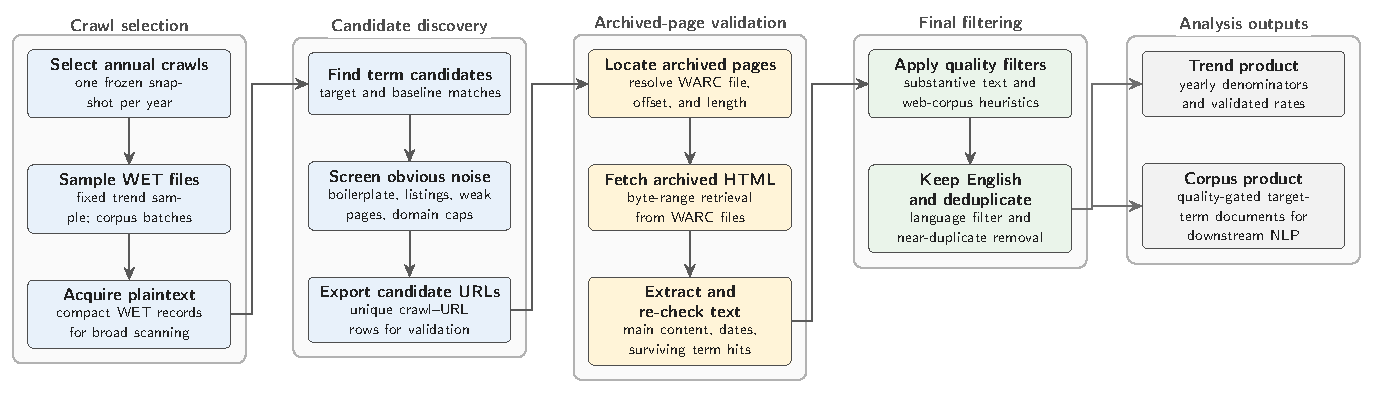
\includegraphics[width=\textwidth]{commoncrawl_pipeline/commoncrawl_collection_pipeline.pdf}
  \caption{Common Crawl collection pipeline used to construct the trend and corpus materials.}
  \label{fig:commoncrawl-pipeline}
\end{figure}
\FloatBarrier

To collect the data for this study, a Common Crawl collection pipeline was developed to extract quality-gated general discourse for the analysis of lexical semantic change (LSC) in specific target terms, here ADHD and autism, against matched baseline terms. The pipeline workflow is illustrated in Figure~\ref{fig:commoncrawl-pipeline}. Target and baseline terms are processed together so that yearly denominators, sampling logic, and quality filters remain comparable across term groups. The pipeline uses Common Crawl's two main file formats sequentially. WET files provide compact extracted plaintext and are therefore used for large-scale term scanning and yearly prevalence denominators, but they lack the HTML structure and metadata needed for stronger boilerplate filtering. Candidate documents are therefore resolved to their corresponding WARC records, which preserve the full HTML code. Although WARC processing is slower, it enables main-text extraction, boilerplate removal, and metadata recovery. This WET-first, WARC-second design keeps the pipeline economical by reserving expensive WARC processing for candidate documents only.\footnote{For a detailed record of the design, configuration, and methodological decisions behind the Common Crawl collection pipeline refer to \url{https://github.com/jako6f/msc-nlp-therapy-speak/blob/main/reports/commoncrawl_corpus_design_and_provenance.md}.}

The design consists of two linked tracks. The trend track uses fixed-effort annual samples to estimate how frequently target and baseline terms appear over time. The corpus track builds a larger, quality-gated document corpus for downstream NLP analysis. As an additional safeguard against overrepresentation by large websites beyond Common Crawl’s restrictive sampling approach, domain caps are applied at 50 WET-validated hit rows per registered domain per Common Crawl crawl. Intermediate summaries and manifests are retained so that each year, crawl, track, and batch remains auditable. The pipeline is designed to run end-to-end on AWS EC2, using S3 as the durable storage and transfer layer for intermediate and final collection artefacts. Yearly crawl selection is deterministic: one Common Crawl snapshot is selected per year near a fixed annual anchor date and then frozen in a crawl map.

Several software choices are methodologically consequential because they affect corpus membership. WET and WARC records are parsed with \texttt{warcio}, WARC pointers are resolved through a local \texttt{pywb}-based index server, archived HTML is converted to main text with Trafilatura and Resiliparse, and post-extraction filtering uses DataTrove quality filters followed by English-language filtering with \texttt{py3langid} \citep{bevendorffElasticChatNoirSearch2018,barbaresiTrafilaturaWebScraping2021,penedoDataTroveLargeScale2026,luiLangidpyOfftheshelfLanguage2012}.\footnote{Both \texttt{warcio} and \texttt{pywb} are open-source Webrecorder projects; see \url{https://github.com/webrecorder/warcio} and \url{https://github.com/webrecorder/pywb}.}

The data collection spans 13 annual Common Crawl snapshots from 2014 to 2026. This window maximises temporal depth while remaining compatible with a stable WET-first, WARC-second workflow. By 2014, Common Crawl provided sufficiently large WET/WARC-format crawls for efficient plaintext scanning, denominator construction, and HTML-based validation; earlier data are less comparable and require additional handling due to older archive formats. The 2026 endpoint reflects the latest collection year available for the project. In the trend track, the pipeline scanned 55.6 million web pages and retained 156,189 pages featuring validated term hits. In the corpus track, it scanned 220 million web pages and retained 336,178 analysis-ready documents. Of these, 87,173 documents contain ADHD or autism target terms. Target membership is non-exclusive: 31,354 documents contain ADHD terms, 67,614 contain autism terms, and 11,795 contain both. The collection was run on an AWS \texttt{m7i-flex.large} instance, featuring 2 vCPUs, 8 GiB of RAM, and up to 12.5 Gbps network bandwidth \citep{CloudComputingServices}. On this instance type, corpus throughput was approximately one hour per million scanned WET records.

\section{Target Terms}

Two target concepts were selected for diachronic semantic analysis: \textit{ADHD} and \textit{autism}. Target documents were retrieved using the matching expressions shown in Table~\ref{tab:target-patterns}. The abbreviation \texttt{ASD} (autism spectrum disorder) was retained only when \textit{autism} occurred within \(\pm 200\) characters, reducing false positives from unrelated acronym use. The acronym \texttt{ADD} (attention deficit disorder) was not included as a matching expression because ADHD is the current canonical diagnostic label, whereas ADD is older and colloquial \citep{americanpsychiatricassociationDiagnosticStatisticalManual2013}; more importantly, \texttt{ADD} would create substantial false positives in WET scanning because it overlaps with the common verb \textit{add} and with web chrome such as ``add to cart''. The broader expression \texttt{attention[-\string\s]?deficit} retains coverage of relevant expanded forms while avoiding this high-noise acronym.

\begin{table}[htbp]
  \centering
  \small
  \caption{Target-term matching expressions.}
  \label{tab:target-patterns}
  \begin{tabular}{@{}ll@{}}
    \toprule
    Concept & Matching expressions \\
    \midrule
    ADHD & \texttt{\string\badhd\string\b}; \texttt{attention[-\string\s]?deficit} \\
    Autism & \texttt{\string\bautism\string\b}; \texttt{\string\bautistic\string\b}; \texttt{autism[-\string\s]?spectrum}; \texttt{\string\bASD\string\b} \\
    \bottomrule
  \end{tabular}
\end{table}

For comparison, three negative, non-clinical emotion terms were selected with sufficient coverage and interpretable usage: \textit{frustration}, \textit{sadness}, and \textit{loneliness}. These terms are not exact semantic controls for ADHD and autism; they provide a baseline for separating target-specific change from broader shifts in negative affective language in the corpus.

\section{Preprocessing}

Following \citet{baesMultidimensionalFrameworkEvaluating2024}, preprocessing was organised around analysis-specific corpus representations rather than a single all-purpose text file. The downstream semantic analyses use a shared mention-level context table built from the extraction pipeline's corpus product. Target and baseline mentions were re-detected using the frozen collection patterns (see Table~\ref{tab:target-patterns}), including the ASD disambiguation rule, and overlapping matches within the same analysis unit were resolved by keeping the longest span. This prevents expressions such as \textit{autism spectrum} from being counted twice as both a phrase and a shorter nested form. Documents containing both ADHD and autism terms were allowed to contribute to both target groups, with separate mention-level contexts emitted for each concept. Same-sentence acronym-and-expansion pairs occurring within a short local window were also collapsed, so cases such as ``attention deficit hyperactivity disorder (ADHD)'' contribute one conceptual ADHD context rather than two near-duplicate rows. To limit domination by repetitive documents while preserving repeated-use signal, each document could contribute at most three mentions per analysis unit. The semantic time variable was then defined as publication year and only contexts with parseable publication dates between 2014 and 2026 were retained for the shared LSC table. This yielded 293,670 mention contexts from 212,651 documents and 135,771 registered domains, including 28,611 ADHD contexts, 68,253 autism contexts, and separate baseline series for frustration, sadness, and loneliness. For each retained mention, the table stores the matched form, raw-form collapse diagnostics, registered domain, publication and crawl metadata, a \(\pm 5\)-token window for affective collocate analyses, and target-sentence passages for breadth and thematic analyses.

\section{NRC--VAD Lexicon}

The affective analyses use the NRC Valence, Arousal, and Dominance (VAD) Lexicon v2.1 \citep{mohammadNRCVADLexicon2025}, rather than the Warriner norms used in SIBling \citep{baesMultidimensionalFrameworkEvaluating2024}. NRC--VAD offers several advantages for the present study. It is substantially larger, providing human ratings for approximately 45,000 English words and 10,000 multi-word phrases, compared with 13,915 words and no phrase entries in Warriner norms. It has also been reported to have higher reliability, with an aggregate reliability estimate of 0.923 across the three VAD dimensions, compared with 0.823 for the Warriner norms.

NRC--VAD scores range from \(-1\) to \(1\). Higher valence scores indicate more positive affect, higher arousal scores indicate greater emotional activation, and higher dominance scores indicate greater perceived control or power. This study uses valence to estimate whether the local contexts of target terms become more positive or negative over time, and arousal to estimate changes in emotional severity. Dominance is included in the source lexicon but is not used in the present analyses. The ratings were produced using Best--Worst Scaling, in which annotators are shown four items and asked to identify the item that best and worst represents the property being rated \citep{mohammadNRCVADLexicon2025}.


\chapter{Methods}
\section{Analytic Overview}

The analysis adapts the SIBling framework of \citet{baesMultidimensionalFrameworkEvaluating2024}, which characterises lexical semantic change along interpretable dimensions rather than treating change as a single aggregate distance. The study estimates five annual trajectories for ADHD and autism discourse: salience, intensity, breadth, sentiment, and thematic content. Salience measures how often target and baseline terms occur in sampled Common Crawl slices. Intensity and sentiment measure the affective arousal and valence of local collocates. Breadth measures contextual dispersion among target-aware embeddings. Thematic evolution identifies the substantive topics that organise target-term contexts over time.

ADHD and autism are analysed as separate conceptual target groups throughout. The raw forms that instantiate each group are retained for diagnostics, but the main estimates are group-level trajectories. The comparator terms \textit{frustration}, \textit{sadness}, and \textit{loneliness} remain separate baseline series rather than being collapsed into a composite baseline. This preserves visibility over broader changes in negative affective language and avoids imposing a single background series unless the comparator trajectories are empirically compatible.

The annual time axis differs by measurement task. Salience uses Common Crawl source year because its denominator is the annual WET scan: documents without candidate term hits do not proceed to WARC extraction or publication-date recovery. All semantic analyses use document publication year, defined as \texttt{lsc\_year}, because the semantic question concerns the date of the discourse rather than the date on which a crawler observed the page. The semantic context table therefore includes only WARC-validated, English-language, deduplicated contexts with parseable publication dates in the 2014--2026 window.

For ADHD and autism, semantic estimates are frame-aware. The main target strata are clinical-only, lived-only, and mixed discourse, together with a duplicated substantive-core aggregate. Non-substantive or insufficient contexts and substantive-other contexts are retained for composition and quality diagnostics but excluded from the main semantic estimates. Baseline terms are not frame-labelled because the clinical versus lived-experience distinction is specific to ADHD/autism discourse.

\section{Frame Classification}

Frame classification is included before the semantic analyses because target-term contexts may change not only in meaning but also in discourse composition. In web text, ADHD and autism may be framed as diagnoses, disorder constructs, service categories, identities, lived experiences, community labels, or incidental boilerplate. Treating all target contexts as one semantic population would risk conflating lexical semantic change with shifts in the prevalence of these frames. This concern follows \citet{pislRevisitingSemanticSeverity2025}, who show that apparent semantic-severity trends can be explained by the changing mental-health context in which a term appears.

The annotation unit is the target sentence plus adjacent sentence context from the shared LSC context table. Each ADHD/autism passage is labelled hierarchically. First, the passage is coded for whether it contains substantive target discourse. Passages that are thin, list-like, navigational, promotional, generic, incidental, noisy, or otherwise insufficient for target-specific interpretation are assigned to the non-substantive or insufficient category. Substantive passages are then coded on two non-exclusive axes: whether clinical framing is present and whether lived-experience framing is present. Clinical framing covers diagnosis, disorder status, symptoms, impairment, treatment, services, medication, research, epidemiology, DSM/ICD-style categories, and educational or clinical support needs. Lived-experience framing covers identity, self-understanding, family or first-person experience, neurodivergent community, masking, stigma, accommodation, everyday coping, belonging, pride, and embodied or social experience.

The two frame axes are converted deterministically into five derived strata. Substantive passages with clinical but not lived-experience framing are labelled clinical-only; passages with lived-experience but not clinical framing are labelled lived-only; passages with both are labelled mixed; and substantive passages with neither are labelled substantive-other. For non-substantive passages, clinical and lived-experience labels are structurally undefined rather than ordinary negative examples.

Labels were produced through a human-led, LLM-assisted annotation procedure. A 200-passage human pilot was used to refine the codebook. A locked version of the codebook was then applied to 3,000 further passages using schema-validated LLM annotation. A separate critic model ranked likely annotation errors; the highest-priority cases and a random residual audit sample were reviewed by the human coder before labels were finalised. Critic suggestions were advisory only: labels changed only when explicitly reviewed by the human coder. This follows the annotator-critic-human-correction logic proposed for efficient LLM-assisted annotation while keeping final adjudication human-controlled \citep{linACTHumanMultimodal2025}.

The corrected labels were used to train a hierarchical classifier over all-MPNET-base-v2 passage embeddings. The classifier uses three balanced logistic-regression heads with standardised features: one head predicts substantive target discourse for all labelled examples, while the clinical and lived-experience heads are trained only on substantive examples. Year, URL, and domain metadata are excluded from the classifier features to reduce leakage from temporal or source-specific artefacts. A separate 200-passage human validation set was held out from codebook development, LLM annotation, criticism, correction, and model training. After validation, the classifier was applied to all ADHD/autism contexts in the shared semantic table, producing hard frame labels and frame probabilities for downstream analysis.

\section{Salience}

Salience estimates the prominence of each analysis unit in annual Common Crawl source-year slices. It is not a semantic measure in itself; rather, it asks whether ADHD- and autism-related terms become more or less frequent in sampled web discourse over time. The primary denominator is the number of tokens in minimum-length WET records entering term matching for year \(Y\). The primary numerator is the number of WARC-validated term hits for analysis unit \(u\). Candidate and WET-validated rates, raw-form composition, publication-year status, and WARC-over-WET retention are retained as diagnostics.

For analysis unit \(u\) and Common Crawl source year \(Y\), salience is defined as

\begin{equation}
\begin{aligned}
\operatorname{Salience}^{\operatorname{WET}}_{u,Y}
&=
\frac{H^{\operatorname{WET}}_{u,Y}}{T_Y}, \\
\operatorname{Salience}^{\operatorname{WARC}}_{u,Y}
&=
\frac{H^{\operatorname{WARC}}_{u,Y}}{T_Y}, \\
\operatorname{Retention}_{u,Y}
&=
\frac{H^{\operatorname{WARC}}_{u,Y}}{H^{\operatorname{WET}}_{u,Y}}.
\end{aligned}
\end{equation}

\noindent Here, \(H^{\operatorname{WET}}_{u,Y}\) is the number of WET-validated hits, \(H^{\operatorname{WARC}}_{u,Y}\) is the number of WARC-validated hits, and \(T_Y\) is the annual scanned-token denominator. Reported salience rates are scaled to hits per million WET tokens. Retention is defined only where \(H^{\operatorname{WET}}_{u,Y} > 0\) and is interpreted as a validation diagnostic rather than as a substantive outcome.

This design follows the relative-frequency logic used by \citet{baesMultidimensionalFrameworkEvaluating2024} while adapting it to the WET-first, WARC-second Common Crawl pipeline. The WARC-validated rate is the primary prominence series because it reflects term survival after full-record validation and main-text extraction. WET and candidate rates remain important for checking whether the validation process changes the temporal pattern.

\section{Sentiment}

Sentiment captures whether the local connotational environment of a target term becomes more positive or more negative over time. Following the collocate-based logic of \citet{baesMultidimensionalFrameworkEvaluating2024}, the measure is computed from words and phrases occurring in a \(\pm 5\)-token window around each target or baseline mention. The present study uses NRC--VAD v2.1 valence scores rather than Warriner norms because NRC--VAD provides broader contemporary English coverage and includes multi-word expressions \citep{mohammadNRCVADLexicon2025}.

The shared context table supplies the mention offsets and \(\pm 5\)-token windows. For each mention, the focal lexical material itself is removed from the scoring window. The remaining context is tokenised and lemmatised with spaCy \texttt{en\_core\_web\_sm}. Punctuation, numerals, and one-character tokens are excluded, but stopwords are retained to keep the collocate index close to the Baes implementation. NRC--VAD entries are normalised with the same lemmatisation procedure. Multi-word expressions are matched greedily before unmatched unigram tokens; if several surface entries collapse to the same lemma phrase, their VAD scores are averaged. The same collocate handoff is reused for intensity so that valence and arousal differ only in the VAD dimension being aggregated.

For analysis unit \(u\), publication year \(Y\), and reported stratum \(s\), annual sentiment is

\begin{equation}
\operatorname{Sentiment}_{u,Y,s}
=
\frac{
\sum_{w \in C_{u,Y,s}} f_{w,u,Y,s} V(w)
}{
\sum_{w \in C_{u,Y,s}} f_{w,u,Y,s}
},
\end{equation}

\noindent where \(C_{u,Y,s}\) is the set of NRC--VAD-matched collocates in the local windows, \(f_{w,u,Y,s}\) is the frequency of collocate \(w\), and \(V(w)\) is its NRC--VAD valence score. Coverage diagnostics record the number of contexts, candidate collocate positions, matched collocate occurrences, unique matched items, and matched-token coverage rate for each unit-year-stratum cell.

\section{Intensity}

Intensity operationalises vertical concept creep as change in the affective arousal of local target contexts. A declining arousal trajectory may be consistent with vertical creep, but it is not interpreted as sufficient evidence on its own because arousal can also reflect advocacy, crisis framing, stigma, newsworthiness, clinical severity, or support-oriented discourse. The measure therefore uses the same local-collocate handoff as Sentiment and differs only in the VAD score being averaged.

Annual intensity for analysis unit \(u\), publication year \(Y\), and reported stratum \(s\) is

\begin{equation}
\operatorname{Intensity}_{u,Y,s}
=
\frac{
\sum_{w \in C_{u,Y,s}} f_{w,u,Y,s} A(w)
}{
\sum_{w \in C_{u,Y,s}} f_{w,u,Y,s}
},
\end{equation}

\noindent where \(A(w)\) is the NRC--VAD arousal score for collocate \(w\). All preprocessing, target-term exclusion, lemmatisation, multi-word matching, frame stratification, and coverage reporting are inherited from the sentiment handoff. This shared preprocessing contract prevents valence and arousal estimates from diverging because of tokenisation or lexicon-matching choices.

\section{Breadth}

Breadth operationalises horizontal concept creep as contextual dispersion: the more diverse the contexts in which a target term appears, the higher its breadth score. \citet{baesMultidimensionalFrameworkEvaluating2024} estimate breadth using sentence-level contextual embeddings. This study replaces a generic sentence-embedding representation with XL-LEXEME, a target-aware word-in-context model designed for lexical semantic change detection \citep{cassottiXLLEXEMEWiCPretrained2023}. The substitution is methodologically important because ADHD, autism, and the baseline terms are analysed as target uses within local passages rather than as undifferentiated sentence topics.

For ADHD and autism, all markable contexts in the three core substantive frames enter the breadth analysis and are also duplicated into the substantive-core aggregate. Baseline terms remain unframed and are deterministically sampled with a cap of 1,000 contexts per baseline-year, stratified by registered domain to limit domination by high-volume websites. Target contexts are not down-sampled, because the target frame strata are the substantive focus and some frame-year cells are comparatively sparse.

Each candidate context is marked with explicit XL-LEXEME target delimiters. The target sentence is used first; if it is too short or the target cannot be marked reliably, the sentence-plus-adjacent context is used. Contexts that cannot be marked are excluded and saved as diagnostics. Identical marked contexts are encoded once and reused through an embedding index. Annual breadth is computed from L2-normalised target-token embeddings using mean pairwise cosine distance.

For analysis unit \(u\), publication year \(Y\), and reported stratum \(s\), with \(N_{u,Y,s}\) contextual embeddings \(\mathbf{v}_1,\ldots,\mathbf{v}_{N_{u,Y,s}}\), breadth is

\begin{equation}
\operatorname{Breadth}_{u,Y,s}
=
\frac{2}{N_{u,Y,s}(N_{u,Y,s}-1)}
\sum_{i=1}^{N_{u,Y,s}-1}
\sum_{j=i+1}^{N_{u,Y,s}}
\left(
1 -
\frac{\mathbf{v}_i \cdot \mathbf{v}_j}
{\lVert \mathbf{v}_i \rVert \lVert \mathbf{v}_j \rVert}
\right).
\end{equation}

\noindent Higher values indicate greater average dissimilarity among target uses in that year and stratum. The implementation uses a closed-form mean-pairwise calculation over normalised vectors for the main score, avoiding the need to materialise all pairwise distances except for diagnostics.

\section{Thematic Evolution}

The thematic analysis is designed as an interpretive layer, not as a scalar semantic-change index. \citet{baesMultidimensionalFrameworkEvaluating2024} include thematic content as a complement to sentiment, intensity, breadth, and salience, using a top-down pathologisation dictionary in their case study. The present study instead uses a bottom-up topic-modelling approach because ADHD/autism discourse is expected to include diagnosis, services, education, workplace accommodation, parenting, neurodiversity, identity, stigma, advocacy, and everyday experience, not only pathologisation.

The modelling unit is a target-centred passage from the shared semantic context table, with frame labels and raw target forms retained as metadata. Text is cleaned minimally to remove obvious boilerplate residue and near-duplicates while preserving lexical content. Topics are estimated using the BERTopic pipeline: embedding, dimensionality reduction, density-based clustering, c-TF-IDF topic representation, and annual topic-prevalence estimation. The principal outputs are topic labels, representative passages, topic prevalence by year, outlier rates, and frame-aware topic summaries where sample size permits. Topic validity is assessed through manual inspection of top terms, representative passages, temporal stability, domain concentration, and whether topics describe target-relevant discourse rather than generic website genres.

\section{Uncertainty, Trend Models, and Diagnostics}

Annual estimates are the primary objects of interpretation. For sentiment, intensity, and breadth, uncertainty intervals are estimated by document-level bootstrap resampling within each analysis-unit, year, and frame-stratum cell, using 500 bootstrap repetitions and the 2.5th and 97.5th percentiles of the bootstrap distribution. The document is the resampling unit because multiple mentions and collocates from the same document are not independent.

Each scalar measure is summarised with a compact annual trend model based on the reporting strategy of \citet{baesMultidimensionalFrameworkEvaluating2024}. For measure \(M\), unit \(u\), year \(Y\), and stratum \(s\), the main descriptive model is

\begin{equation}
M_{u,Y,s}
=
\alpha_{u,s}
+
\beta_{u,s}(Y - \bar{Y})
+
\varepsilon_{u,Y,s},
\end{equation}

\noindent where \(\beta_{u,s}\) is the annual linear slope and \(\bar{Y}\) is the centre of the observed year range. The trend tables record the slope per year, standard error, \(p\)-value, adjusted \(R^2\), standardised year coefficient, and a residual autocorrelation diagnostic. Because the annual series span only 13 years and are further stratified by frame for ADHD and autism, these models are treated as descriptive summaries of direction and strength rather than as causal or population-level time-series tests.

Residual autocorrelation is checked with a Durbin--Watson-style diagnostic. When a scalar series is flagged, an AR(1)-transformed sensitivity slope is reported in the corresponding trend table; otherwise the ordinary least-squares estimate remains the main summary. Quadratic fits are retained only as diagnostics for visibly curved trajectories and are not used as the default model.

All downstream analyses carry diagnostic tables alongside the main estimates. These include annual sample size, document and domain counts, raw-form composition, low-volume frame-year flags, VAD coverage, top contributing collocates, WARC retention for salience, and domain-concentration checks where available. Frame-specific target estimates are flagged when they contain fewer than 100 contexts or fewer than 50 documents. These diagnostics do not automatically exclude observations, but they determine how cautiously individual annual points or frame-specific trends should be interpreted.


\chapter{Results}
% Results section reserved for final diachronic findings.
Table~\ref{tab:lsc-classification-validation} reports the held-out validation performance of the hierarchical frame classifier used to stratify ADHD/autism target contexts. The clinical and lived-experience rows evaluate the Stage-1 frame heads among passages marked as substantive target discourse in the human validation labels.

\begin{table}[htbp]
\centering
\caption{Held-out validation performance for the hierarchical frame classifier.}
\label{tab:lsc-classification-validation}
\small
\begin{tabular}{@{}lcccccc@{}}
\toprule
Validation target & Support & Precision & Recall & F1 & Accuracy & Bal. acc. \\
\midrule
Substantive target discourse & 141/200 & .887 & .837 & .861 & .810 & .791 \\
Clinical framing & 105/141 & .903 & .886 & .894 & .844 & .804 \\
Lived-experience framing & 46/141 & .704 & .826 & .760 & .830 & .829 \\
\bottomrule
\end{tabular}
\parbox{\linewidth}{\footnotesize Note. Support gives positive cases over the validation denominator. Substantive target discourse is evaluated on all 200 held-out passages. Clinical and lived-experience rows report Stage-1 head performance among the 141 passages marked as substantive target discourse in the human validation labels.}
\end{table}


As shown in Table~\ref{tab:lsc-regression-target-frames}, the target trend models summarise the annual ADHD and autism trajectories by frame. The salience rows are source-year models, while the semantic rows use document publication year.

\begin{table}[htbp]
\centering
\caption{Descriptive annual trend models for ADHD and Autism LSC trajectories by frame.}
\label{tab:lsc-regression-target-frames}
\scriptsize
\begin{tabular}{@{}lllccc@{}}
\toprule
Measure & Target & Frame & $B(SE)$ & $\beta$ & Adj. $R^2$ \\
\midrule
Salience & ADHD & Overall & $0.0073$ (0.0043) & 0.46 & 0.14 \\
Salience & Autism & Overall & $-0.0228^{*}$ (0.0087) & -0.62 & 0.33 \\
Sentiment & ADHD & Overall & $0.0023^{\dagger}$ (0.0014) & 0.46 & 0.14 \\
Sentiment & ADHD & Clinical & $0.0013^{\dagger}$ (0.0015) & 0.24 & -0.03 \\
Sentiment & ADHD & Lived experience & $0.0002$ (0.0017) & 0.03 & -0.09 \\
Sentiment & Autism & Overall & $0.0012$ (0.0006) & 0.50 & 0.18 \\
Sentiment & Autism & Clinical & $0.0022^{\dagger}$ (0.0015) & 0.42 & 0.10 \\
Sentiment & Autism & Lived experience & $-0.0038$ (0.0022) & -0.46 & 0.14 \\
Intensity & ADHD & Overall & $0.0001$ (0.0005) & 0.04 & -0.09 \\
Intensity & ADHD & Clinical & $0.0002$ (0.0006) & 0.10 & -0.08 \\
Intensity & ADHD & Lived experience & $0.0015$ (0.0009) & 0.45 & 0.13 \\
Intensity & Autism & Overall & $0.0011$ (0.0008) & 0.36 & 0.05 \\
Intensity & Autism & Clinical & $0.0010^{*}$ (0.0004) & 0.56 & 0.25 \\
Intensity & Autism & Lived experience & $0.0025$ (0.0021) & 0.34 & 0.04 \\
Breadth & ADHD & Overall & $-0.0020^{***}$ (0.0003) & -0.89 & 0.77 \\
Breadth & ADHD & Clinical & $-0.0018^{***}$ (0.0003) & -0.85 & 0.69 \\
Breadth & ADHD & Lived experience & $-0.0004^{\dagger}$ (0.0006) & -0.18 & -0.06 \\
Breadth & Autism & Overall & $0.0001^{\dagger}$ (0.0002) & 0.14 & -0.07 \\
Breadth & Autism & Clinical & $0.0007^{*\dagger}$ (0.0003) & 0.58 & 0.28 \\
Breadth & Autism & Lived experience & $-0.0010^{*}$ (0.0004) & -0.60 & 0.30 \\
\bottomrule
\end{tabular}
\parbox{\linewidth}{\footnotesize Note. Cells report annual unstandardised OLS slopes as $B(SE)$; $\beta$ is the standardised year coefficient. Salience uses Common Crawl source year and has only an overall target row; semantic measures use document publication year. Significance markers: $^{*}p<.05$, $^{**}p<.01$, $^{***}p<.001$. $^{\dagger}$ indicates a residual-autocorrelation flag; AR(1) sensitivity estimates for flagged rows are reported in Appendix Table~\ref{tab:lsc-ar1-sensitivity-flagged}. P values are descriptive and uncorrected.}
\end{table}



\chapter{Discussion}
This study asked whether ADHD and autism---two diagnostic concepts at the centre of contemporary debates about the popularisation of mental health language---have undergone the semantic loosening that concept creep theory predicts, and it did so in general web discourse rather than in the curated corpora on which prior evidence largely rests. The answer, on the measures used here, is that they have not. Across a frame-aware adaptation of the SIBling framework \citep{baesMultidimensionalFrameworkEvaluating2024}, the dominant empirical signature was not milder, broader, or diluted meaning, but a reorganisation of the discourse surrounding two comparatively stable concepts. This chapter first summarises the findings in relation to the research questions (Section~\ref{sec:discussion-summary}). It then develops three interpretive claims: that the results indicate semantic consolidation rather than concept creep (Section~\ref{sec:discussion-semantic-consolidation}); that the clearest change in ADHD and autism discourse over the period was compositional---a shift from disorder talk toward lived experience, accompanied by a recent positification (a positive valence shift) of clinical contexts (Section~\ref{sec:discussion-lived-experience}); and that the robustness checks expose a measurement sensitivity with implications for the wider literature on lexical semantic change (Section~\ref{sec:discussion-measurement-sensitivity}). Limitations (Section~\ref{sec:discussion-limitations}) and directions for future research (Section~\ref{sec:discussion-future-research}) close the chapter.

\section{Summary of Findings}
\label{sec:discussion-summary}

With respect to RQ1, ADHD and autism did not become jointly more prominent in sampled general web discourse between 2014 and 2026. Autism salience declined by a fitted 28.9\%, while the fitted 27.0\% increase for ADHD did not differ from zero at the uncorrected \(p < .05\) level. The comparators moved in different directions---loneliness rose, sadness fell, and frustration showed no reliable trend---so the autism decline cannot be attributed to a uniform contraction of negative-affect language in the crawl.

With respect to RQ2, the balance of framing shifted toward lived experience. Among contexts assigned to a single clear frame, the lived-experience share of ADHD discourse rose by 1.07 percentage points per year, a fitted increase from 17.5\% to 30.3\%; the corresponding autism trend was directionally similar but roughly half the size and was not retained by the AR(1) sensitivity model. The full predicted composition showed the same pattern, with clinical-only shares falling for both targets.

With respect to RQ3, neither of the hypothesised forms of concept creep was supported (Table~\ref{tab:lsc-regression-target-frames}). Contrary to the vertical-creep hypothesis, intensity did not decline in any target stratum; the only slope that differed from zero was a nominal increase in autism clinical contexts. Contrary to the horizontal-creep hypothesis, breadth under the target-aware operationalisation decreased for ADHD overall and in ADHD clinical contexts---the strongest semantic trends observed in the study---decreased in autism lived-experience contexts, and was flat for autism overall, with the nominally positive autism clinical slope not surviving the AR(1) check. Sentiment showed no linear trend in any target stratum; instead, the autocorrelation-flagged series traced U-shaped trajectories with minima between mid-2018 and mid-2019, and the AR(1) sensitivity model indicated a positive valence trend in autism clinical contexts.

With respect to RQ4, the thematic content of both discourses changed remarkably little. The 28 neighbours retained by the stability filter were diagnostic and child- or family-centred throughout: \emph{child}, \emph{disorder}, \emph{symptom}, \emph{diagnose}, and \emph{condition} anchored ADHD discourse, while \emph{child} remained the highest-similarity neighbour of autism overall and in clinical contexts, with \emph{people}, \emph{support}, \emph{life}, and \emph{family} characterising lived-experience contexts.

\section[Semantic Consolidation Rather than Concept Creep]{Semantic Consolidation Rather than Concept\texorpdfstring{\\}{ }Creep}
\label{sec:discussion-semantic-consolidation}

The central substantive finding is a double null with a directional surprise. ADHD and autism did not drift into less emotionally intense contexts, and they did not disperse across a broader range of lexical contexts; where reliable movement occurred, it ran in the opposite direction, most clearly in the sustained contraction of ADHD breadth, under the target-aware operationalisation, from .138 to .117. This pattern is unlikely to reflect measures that were simply too blunt to register change of any kind: the same instruments detected reliable trends among the comparators, including a broadening of frustration, an intensification of sadness contexts, and robust positification of frustration and loneliness. Within this corpus and this measurement scheme, the affective and contextual profiles of ADHD and autism were among the more stable series observed.

This stability is intelligible in light of \citeauthor{iacobComputationalAnalysisEmergence2026}'s \citeyear{iacobComputationalAnalysisEmergence2026} finding that long-established, codified psychological terms such as \emph{OCD} and \emph{bipolar} showed little year-to-year semantic movement on Reddit, whereas newer vernacular terms such as \emph{gaslighting} shifted substantially. ADHD and autism are institutionally anchored concepts: their reference is stabilised by diagnostic manuals, clinical gatekeeping, service categories, and educational law in ways that ordinary-language harm concepts such as \emph{bullying} or \emph{harassment} \citep{vylomovaSemanticChangesHarmrelated2021} are not. Concept creep in such categories may therefore operate primarily at the level of diagnostic criteria and category application---who is counted as an instance---rather than at the level of the contexts in which the label is used. This reading is consistent with \citeauthor{fabianoDiagnosticInflationDSM2020}'s \citeyear{fabianoDiagnosticInflationDSM2020} meta-analytic evidence that ADHD's diagnostic criteria inflated substantially across successive DSM revisions, and it suggests a distinction the concept creep literature has tended to elide: a category can expand extensionally, absorbing many more people, while the typical linguistic contexts of its name---which is all that collocate- and embedding-based measures index---remain stable or even converge. On this account, the rising prevalence documented in the epidemiological literature
\citep{zeidanGlobalPrevalenceAutism2022,mckechnieAttentiondeficitHyperactivityDisorder2023,cuiDSM5ChangesCOVID192026} need not leave the semantic trace that a naive application of concept creep theory would predict.

The ADHD breadth contraction invites a further interpretation: consolidation of a discourse genre. As ADHD moved from a specialist topic to a mainstream one, its web coverage appears to have converged on a recognisable register---symptom lists, awareness explainers, parenting and educational advice---rather than diversifying. The post-hoc diagnostics support this reading: the highest-distance ADHD contexts remained saturated with diagnostic and educational vocabulary (\emph{disorder}, \emph{impulsivity}, \emph{inattention}, \emph{learning}, \emph{dyslexia}), and the stable neighbours were uniformly diagnostic and child-related. Alternatively, the contraction may reflect the composition of the sample rather than the concept: if health articles written to a common template (e.g., for search-engine optimisation) account for a growing share of retained ADHD documents, their near-identical contexts would pull measured breadth down even if the meaning of ADHD itself were unchanged. The two possibilities are compatible and cannot be separated here. Either way, the frustration comparator's concurrent broadening indicates that the contraction is target-specific rather than a corpus-wide artefact.

The findings also bear on the evidentiary question that motivated the study. Prior evidence for creep in mental-health-related concepts derives largely from psychology abstracts and curated general-language corpora \citep{vylomovaSemanticChangesHarmrelated2021,baesSemanticShiftsMental2023,baesSemanticInflationTrauma2023}, and \citet{pislRevisitingSemanticSeverity2025} have shown that apparent semantic trends in such corpora can be artefacts of shifting discourse composition. The present study addressed both concerns---moving to general web discourse and stratifying by frame---and found no concept creep in ADHD and autism. This does not overturn earlier findings for other concepts, which concerned different terms with different institutional standing, but it does reinforce the conclusion that creep results are corpus- and composition-dependent, and that inferences about cultural change drawn from any single curated corpus should be made cautiously. At the same time, Common Crawl imposes structural constraints of its own \citep{baackCriticalAnalysisLargest2024}, a point developed in Section~\ref{sec:discussion-limitations}; the discrepancy between corpora identifies corpus dependence rather than settling which corpus better reflects the underlying culture.

The salience results sharpen this point. Autism's declining prominence in the sampled crawl sits awkwardly beside steeply rising diagnosed prevalence \citep{zeidanGlobalPrevalenceAutism2022,abs2024} and more than four million TikTok videos hashtagged by June 2026. The most plausible reconciliation is that this discourse growth is concentrated on social platforms and behind robots.txt restrictions, both largely outside Common Crawl's reach \citep{baackCriticalAnalysisLargest2024}: ``web discourse'' is not a single population, and the discourse boom visible on TikTok is not automatically visible---or even present---in web-scale archives.

\section{From Disorder Talk to Lived Experience}
\label{sec:discussion-lived-experience}

If the meanings of ADHD and autism held broadly steady, the way they are talked about did not. The most reliable change detected in the entire study concerns who and what these terms are used to discuss: ADHD discourse shifted markedly from clinical toward lived-experience framing, and autism discourse moved in the same direction from a substantially higher starting point (a fitted 35.9\% lived-experience share in 2014, against 17.5\% for ADHD). This asymmetry is theoretically coherent. Identity-first and community framings of autism were established well before the study window, whereas ADHD's popular turn---adult self-recognition, online community formation, and identity-oriented content---is more recent, consistent with qualitative evidence on ADHD online communities \citep{ginappExperiencesAdultsADHD2023}, clinical reports of self-diagnosed presentations \citep{hartnettSocialMediaADHD2024}, the sharp growth in ADHD media coverage \citep{martinChangingPrevalenceADHD2025}, and accounts of ``platformed diagnosis'' spilling outward from social media \citep{alperTikTokAlgorithmicallyMediated2025}. On this reading, ADHD is undergoing in the 2020s a reframing that autism discourse partially completed earlier, leaving autism's trend flatter and, after accounting for serial dependence, statistically unresolved.

The compositional shift also vindicates the study's frame-aware design on its own terms. Frame-specific trajectories repeatedly diverged in sign: autism clinical breadth trended nominally upward while lived-experience breadth declined; autism clinical sentiment was positive under the AR(1) model while the lived-experience slope pointed downward. An unstratified analysis would have blended these movements with the changing frame mixture, precisely the conflation that \citet{pislRevisitingSemanticSeverity2025} identified in newspaper text. The present results extend that demonstration to web-scale data and to a different kind of composition problem. For anxiety and depression, stratification must first separate clinical constructs from the ordinary states and non-clinical phenomena (e.g., everyday anxiety, or an economic depression) the same words denote \citep{xiaoHaveConceptsAnxiety2023}; ADHD and autism are diagnostic concepts by definition, so the composition that shifts is the framing of the diagnosis itself---as disorder construct or as identity and lived experience.

The sentiment results add a temporal texture that linear models missed. The flagged ADHD and autism clinical series traced U-shapes with minima between Q3 2018 and Q2 2019, implying declining valence through the mid-2010s followed by recovery through 2026, with the autism clinical positification robust to first-order autocorrelation. The turning point falls within the period in which neurodiversity entered mainstream media vocabulary, with US news coverage of neurodiversity and neurodivergent individuals increasing between 2016 and 2022 \citep{huang-horowitzExploringMediaDiscourse2025}, and in which first-person ADHD and autism content proliferated on social platforms \citep{hartnettSocialMediaADHD2024,alperTikTokAlgorithmicallyMediated2025}. The post-hoc contributors indicate that the recovery is carried by child-, family-, and support-related vocabulary against a persistent background of diagnostic and comorbidity terms. Even so, this is at most gentle destigmatisation, and it is not uniform: the appearance of \emph{dangerous} and \emph{obsession} among the late-period arousal-raising collocates in autism lived-experience contexts shows that alarmed or stigmatising discourse persists.

A further pattern deserves note. From 2018 onward, \emph{adhd} entered the leading negative-valence contributors in autism contexts, mirroring the persistent presence of \emph{autism} in ADHD contexts, and 11,795 corpus documents contained both targets. This is web-general corroboration of the ADHD--autism semantic convergence that \citet{kangConvergingRepresentationsAttentionDeficit2025} reported on Reddit from 2019: the two concepts are increasingly discussed together, as co-occurring conditions and as jointly constitutive of neurodivergent identity. The convergence also complicates target-specific measurement, since each concept increasingly forms part of the other's context.

Taken together, these results speak to the therapy-speak debate with which this project opened. The trivialisation concern holds that popularisation erodes the meaning of clinical terms, dispersing them across ever milder and more heterogeneous uses and thereby depriving diagnosed people of precise language for their experiences \citep{isern-masUnmaskingTherapyspeak2025,spencerIsntEveryoneLittle2021}. For ADHD and autism in general web discourse, the semantic preconditions of that concern are not in evidence: contexts did not become milder, did not broaden, and remained thematically anchored to diagnosis, childhood, and family. A different hermeneutical concern, however, does find support: despite the steep rise in adult diagnoses \citep{mckechnieAttentiondeficitHyperactivityDisorder2023}, the stable thematic core of both discourses remained resolutely child-centred, suggesting that late-diagnosed adults continued to encounter a web discourse organised around children's presentations rather than their own.

\section[Measurement Sensitivity and Its Implications for LSC Research]{Measurement Sensitivity and Its Implications for\texorpdfstring{\\}{ }LSC Research}
\label{sec:discussion-measurement-sensitivity}

The robustness checks carry an implication that extends beyond this study. Substituting the original SIBling resources for the refined ones changed some substantive conclusions. Under Warriner norms, ADHD intensity declined reliably, a result that, taken alone, would have been reported as vertical concept creep---whereas the NRC--VAD estimate was flat. Under MPNet sentence embeddings, the pronounced XL-LEXEME decline in ADHD breadth attenuated to a null, while autism's flat XL-LEXEME trajectory became a reliable MPNet decline. Two conclusions were common to both operationalisations and can be stated with corresponding confidence: neither target broadened horizontally, and neither showed a reliable linear sentiment trend. The vertical-creep conclusion, by contrast, is measurement-conditional and should be reported as such.

There are principled grounds for preferring the refined measures \textit{a priori}: NRC--VAD offers roughly threefold lexical coverage, multi-word entries, and higher reported reliability \citep{mohammadNRCVADLexicon2025}, and XL-LEXEME is a word-in-context model built for LSC detection that represents the target use itself rather than the surrounding sentence topic \citep{cassottiXLLEXEMEWiCPretrained2023}, a distinction that matters when the analytic object is a term's usage rather than a document's subject matter. But the \textit{a priori} argument does not dissolve the empirical problem: the SIBling dimensions, as currently operationalised, are not measurement-invariant, a possibility its authors anticipated in describing the operationalisations as first implementations \citep{baesMultidimensionalFrameworkEvaluating2024}. This observation may also help explain the mixed findings accumulating in the literature---increases in semantic intensity where creep predicts decreases \citep{xiaoHaveConceptsAnxiety2023}, reversals across corpora \citep{iacobComputationalAnalysisEmergence2026}, and composition-dependent trends \citep{pislRevisitingSemanticSeverity2025}---some portion of which plausibly reflects instrumentation rather than substance. Until the framework's dimensions are validated against human judgements of intensity, breadth, and connotation, LSC studies in this tradition would do well to treat multi-resource robustness checks not as optional supplements but as part of the primary analysis, as practised here.

\section{Limitations}
\label{sec:discussion-limitations}

The most consequential limitations concern the corpus. Common Crawl is neither a complete copy of the web nor a representative sample of it: domain selection follows harmonic centrality, adopted in 2017 (prior crawls relied mainly on externally donated URL seed lists, which had dwindled over time); major social platforms are absent; and rights-holder blocking via robots.txt has grown over precisely the years studied \citep{baackCriticalAnalysisLargest2024}. Temporal comparability is therefore imperfect, and trends---salience above all---partly reflect changes in what the crawl could see. Findings generalise to quality-filtered, English-language open-web discourse as archived by Common Crawl, not to public discourse at large, and emphatically not to the social platforms where much contemporary ADHD and autism discourse occurs.

The frame-aware design inherits classifier error. The lived-experience head performed adequately but weakest (F1 = .760, precision = .704), so lived-experience strata contain clinical admixture, which will have attenuated frame contrasts and blurred frame-specific trends. The more damaging possibility is non-stationary error: stylistic drift inflating late-period lived-experience false positives would manufacture exactly the trend observed. A period-stratified audit found no evidence of this---lived-experience precision and calibration were best in the late period, and human-authoritative labels on the adjudicated passages reproduce the rise independently of the classifier---though with only 11--23 lived-experience validation positives per period, modest error drift cannot be excluded, and the fitted ADHD rise may be somewhat smaller than the apparent 12.8 percentage points. The human gold standard also rests on a single coder: the pilot, the adjudication of flagged cases, and the 200-passage validation set reflect one annotator's judgement, so no inter-annotator agreement can be reported and validation performance is measured against an individual rather than a consensus standard. And although the ACT workflow retained human authority over labels, LLM-assisted annotation may import model-specific biases that human review of high-risk cases only partially corrects. The frame codebook, finally, is specific to ADHD and autism, so the baselines could not be frame-stratified, limiting target–baseline comparisons to unframed series.

Three further limitations should be explicit. The affective measures score lemmatised collocates with context-free lexicon values within the \(\pm\)5-token windows adopted from the SIBling operationalisation \citep{baesMultidimensionalFrameworkEvaluating2024}, and are therefore blind to negation, irony, and syntactic scope. The comparators are baselines for general negative-affect language, not matched semantic controls. And the design as a whole is observational: it can characterise how discourse changed, but not why. The inferential bounds set out in Section~\ref{sec:methods-statistical-analysis}---34 uncorrected trend tests and the minimum detectable effects implied by 13 annual observations---apply to all null results reported here.

\section{Directions for Future Research}
\label{sec:discussion-future-research}

Three extensions follow directly. First, cross-platform designs are needed to test the suggestion advanced in Section~\ref{sec:discussion-semantic-consolidation} that ADHD and autism discourse has migrated toward social platforms outside Common Crawl's reach: applying the same frame-aware measures to web, Reddit, and short-video corpora over a common window would show whether the semantic stability observed here coexists with creep in platform discourse \citep[cf.][]{devriesExploringConceptCreep2025,aragon-guevaraReachAccuracyInformation2025}. Second, the measurement sensitivity identified in Section~\ref{sec:discussion-measurement-sensitivity} motivates validation studies in which lexicon- and embedding-based intensity, breadth, and sentiment estimates are benchmarked against human judgements of the same contexts, so that resource choice can rest on demonstrated convergent validity rather than plausibility arguments. Third, the substantive account developed here generates testable expectations: if institutional codification protects diagnostic labels from creep, then frame-aware analyses of less codified neighbouring vocabulary---\emph{neurodivergent}, \emph{masking}, \emph{stimming}, \emph{executive dysfunction}---should reveal greater semantic movement than ADHD and autism themselves; and linking annual discourse measures to diagnostic and prescribing statistics would allow the temporal ordering assumed by the prevalence inflation hypothesis \citep{foulkesAreMentalHealth2023} to be examined directly. Finer-than-annual time resolution, non-English web discourse, and qualitative analysis of the contentious late-period lived-experience contexts flagged in Section~\ref{sec:discussion-lived-experience} would each add further resolution to the picture drawn here.


\chapter{Conclusion}
This research project examined lexical semantic change in ADHD and autism across thirteen years of general web discourse, motivated by the concern that the popularisation of mental health language erodes the meaning of the terms on which diagnosed people rely. It constructed a reproducible Common Crawl pipeline spanning 2014--2026, separated clinical from lived-experience framing with a validated hierarchical classifier, and estimated salience, sentiment, intensity, breadth, and thematic-neighbour trajectories using a refined adaptation of the SIBling framework, benchmarked against the framework's original operationalisations.

The hypothesised concept creep did not materialise. ADHD and autism did not drift into milder emotional contexts, and their contexts did not broaden; ADHD contexts contracted markedly, and the thematic core of both discourses---diagnosis, childhood, family---remained stable throughout. What changed was the composition of the discourse: a robust shift from clinical toward lived-experience framing, strongest for ADHD, together with a recent, tentative positification of clinical contexts and growing entanglement between the two concepts. In sampled open-web discourse, autism became less prominent rather than more, underscoring that the contemporary surge in ADHD and autism talk is unevenly distributed across the digital landscape.

The study makes four contributions. Substantively, it extends concept creep and therapy-speak research to ADHD and autism and provides evidence that two institutionally codified diagnostic concepts resisted the semantic loosening documented for ordinary-language harm concepts, with category expansion proceeding through application rather than through the dilution of meaning in use. Evidentially, it moves LSC research on mental-health concepts from curated corpora to general web discourse and shows that conclusions do not simply transfer between the two. Analytically, it demonstrates at web scale that discourse composition and semantic change must be separated, since frame-specific trajectories repeatedly diverged from aggregates. Methodologically, its robustness checks show that key SIBling conclusions are conditional on lexicon and encoder choice, identifying measurement validation as a priority for the field.

The broader implication is a reframing of the trivialisation concern. For ADHD and autism on the open web, the words have largely held their shape; it is the conversation around them---who speaks, in what frame, and on which platforms---that has been transformed. Whether the same holds where that conversation is now loudest remains the question this project leaves open, and the tools it provides are designed to answer it.


% =============================================================================
% References
% =============================================================================
\backmatter
\renewcommand{\bibname}{References}
\phantomsection
\addcontentsline{toc}{chapter}{References}
\bibliographystyle{bibs/compling}
\bibliography{bibs/msc-nlp-therapy-speak}

% =============================================================================
% Appendices (optional)
% =============================================================================
\appendix
\chapter{Appendices}
\section{Baseline Comparator Trend Models}

Table~\ref{tab:lsc-regression-baseline-comparators} reports the unframed comparator-term trend models used to contextualise the ADHD and autism target trajectories.

\begin{table}[htbp]
\centering
\caption{Descriptive annual trend models for baseline comparator trajectories.}
\label{tab:lsc-regression-baseline-comparators}
\small
\begin{tabular}{@{}llccc@{}}
\toprule
Measure & Comparator & $B(SE)$ & $\beta$ & Adj. $R^2$ \\
\midrule
Salience & frustration & $-0.0175^{\dagger}$ (0.0167) & -0.30 & 0.01 \\
Salience & loneliness & $0.0056^{*}$ (0.0021) & 0.62 & 0.33 \\
Salience & sadness & $-0.0171^{**}$ (0.0039) & -0.80 & 0.61 \\
Sentiment & frustration & $0.0037^{*\dagger}$ (0.0013) & 0.67 & 0.39 \\
Sentiment & loneliness & $0.0044^{**\dagger}$ (0.0013) & 0.71 & 0.45 \\
Sentiment & sadness & $-0.0030^{**}$ (0.0007) & -0.79 & 0.59 \\
Intensity & frustration & $-0.0004^{\dagger}$ (0.0006) & -0.23 & -0.03 \\
Intensity & loneliness & $-0.0006$ (0.0006) & -0.30 & 0.01 \\
Intensity & sadness & $0.0028^{***}$ (0.0004) & 0.88 & 0.76 \\
Breadth & frustration & $0.0020^{**}$ (0.0006) & 0.72 & 0.48 \\
Breadth & loneliness & $-0.0007$ (0.0004) & -0.51 & 0.19 \\
Breadth & sadness & $-0.0010^{**\dagger}$ (0.0003) & -0.71 & 0.46 \\
\bottomrule
\end{tabular}
\parbox{\linewidth}{\footnotesize Note. Cells report annual unstandardised OLS slopes as $B(SE)$; $\beta$ is the standardised year coefficient. Comparator terms are unframed baseline series. Salience uses Common Crawl source year and semantic measures use document publication year. Significance markers: $^{*}p<.05$, $^{**}p<.01$, $^{***}p<.001$. $^{\dagger}$ indicates a residual-autocorrelation flag; AR(1) sensitivity estimates for flagged rows are reported in Appendix Table~\ref{tab:lsc-ar1-sensitivity-flagged}. P values are descriptive and uncorrected.}
\end{table}


\section{Quadratic Trend Diagnostics}

Table~\ref{tab:lsc-quadratic-diagnostics} reports the diagnostic quadratic models for annual LSC trajectories whose linear residual diagnostics were flagged for autocorrelation.

\begin{table}[htbp]
\centering
\caption{Supplementary quadratic models for autocorrelation-flagged LSC trajectories.}
\label{tab:lsc-quadratic-diagnostics}
\scriptsize
\begin{tabular}{@{}lllcccc@{}}
\toprule
Measure & Target & Frame & Linear $B(SE)$ & Quadratic $B_2(SE)$ & $\Delta$ Adj. $R^2$ & Vertex \\
\midrule
Breadth & Autism & Overall & $0.0001$ (0.0002) & $-0.0002^{**}$ (0.0000) & 0.58 & April 2020 (inverted U) \\
Breadth & Autism & Clinical & $0.0007^{*}$ (0.0003) & $-0.0003^{***}$ (0.0001) & 0.51 & May 2021 (inverted U) \\
Sentiment & ADHD & Clinical & $0.0004$ (0.0009) & $0.0007^{**}$ (0.0002) & 0.60 & September 2019 (U) \\
Sentiment & Autism & Clinical & $0.0012$ (0.0009) & $0.0007^{**}$ (0.0002) & 0.61 & March 2019 (U) \\
\bottomrule
\end{tabular}
\parbox{\linewidth}{\footnotesize Note. Rows are restricted to annual series whose linear-model residuals were flagged for autocorrelation. Linear $B$ is the annual OLS slope from the primary trend model. Quadratic $B_2$ is the centred-year-squared coefficient; $\Delta$ Adj. $R^2$ is the adjusted-$R^2$ gain over the linear model. Vertex labels give the calendar month containing the fitted decimal-year vertex; the underlying observations are annual. Significance markers are descriptive and uncorrected: $^{*}p<.05$, $^{**}p<.01$, $^{***}p<.001$.}
\end{table}



\end{document}
